\chapter[Embasamento Teórico]{Embasamento Teórico}
\label{ch:cap2}
O \textit{Power Monitor} surgiu da necessidade da conscientização do gasto energético e da melhor compreensão da conta de luz. Baseado nesse conceito,
foi desenvolvido um \textit{software} que permite uma fácil comunicação com qualquer equipamento construído que tenha a finalidade de monitorar a energia elétrica e um \textit{hardware} para demonstração
da comunicação entre ambos.
O sistema traz uma forma mais fácil e próxima do consumidor final de se quantificar a energia elétrica consumida em um estabelecimento. No lugar do quilowatt-hora, medida usada atualmente,
o \textit{software} propõe mensurar o gasto energético em reais (R\$), trazendo a realidade do consumo mensal.

Este capítulo trará os conceitos essenciais para o entendimento do trabalho, descrevendo todas as tecnologias utilizadas no desenvolvimento 
do \textit{Power Monitor}.

\section[\textit{Ferramentas e linguagens}]{\textit{Ferramentas e linguagens}}\label{ferramenta-linguagem}
No decorrer do desenvolvimento do \textit{software} fez-se uso de algumas tecnologias e linguagens de programação que serão descrita a seguir.
\subsection[\textit{Node.js}]{\textit{Node.js}}\label{node}
Node.js é um \textit{framework}, interpretador do código JavaScript (\autoref{js}), com o foco do uso da linguagem do lado do cliente para servidores. Com um objetivo simples
que é ajudar desenvolvedores na criação de aplicações de alta escalabilidade, com códigos capazes de administrar e manipular várias conexões simultaneamente
em um único servidor. O \textit{Node.js} é baseado na \textit{runtime} V8 \textit{JavaScript Engine}. Foi desenvolvido por Ryan Danhl em 2009, e o seu desenvolvimento
é mantido pela fundação \textit{Node.js} e \textit{Linux Foundation} \cite{ref-nodejs}. 
\subsection[\textit{JavaScript}]{\textit{JavaScript}}\label{js}
JavaScript é uma linguagem de programação interpretada de alto nível, juntamente com HTML e CSS é uma das linguagens mais utilizadas no mundo \textit{web}.
Após o uso da linguagem as páginas \textit{web} começaram a ter uma maior interatividade com o usuário. A grande maioria dos \textit{browsers} tem um
mecanismo de compilação dedicado para o JavaScript \cite{ref-js}. Por ser uma linguagem multi-paradigma o JavaScript suporta paradigmas funcionais, orientados a eventos 
e até mesmo paradigmas de orientação a objeto.
Inicialmente era usada apenas no lado do cliente em \textit{web browsers}, mas atualmente está presente em vários outros tipos de \textit{softwares} incluindo
servidores - como já foi discutido na \autoref{node} - \textit{databases} e até sistemas \textit{desktop} como os leitores de PDF, programas de música e recentemente
vem ganhando espaço no desenvolvimento de aplicativos para celular \cite{ref-jsmobile}.

\subsection[\textit{WebSocket}]{\textit{WebSocket}}\label{websocket}
A ideia da tecnologia surgiu da problemática onde as comunicações entre servidor e aplicação eram baseadas na sobrecarga do HTTP, que não é indicado para aplicações
de baixa latência. O WebSocket pode ser definido como uma API que estabelece a conexão entre aplicação e servidor. Resumidamente é uma conexão, baseada no protocolo TCP, persistente
entre servidor e cliente onde ambas as partes podem enviar ou receber informações. A forma como a conexão acontece é simples:
o cliente e o servidor antes de tudo devem negociar o \textit{handshake}, que segundo \cite{ref-handshake} é o precesso pelo qual duas máquinas afirmam uma a outra que a reconheceu e está pronta para iniciar a comunicação.
No momento em que a negocição é confirmada a conexão é establecida, criando um canal de comunicação bidirecional. A \autoref{fig:websocket-diagram} retrata o cenário descrito.

\begin{figure}[h!]
	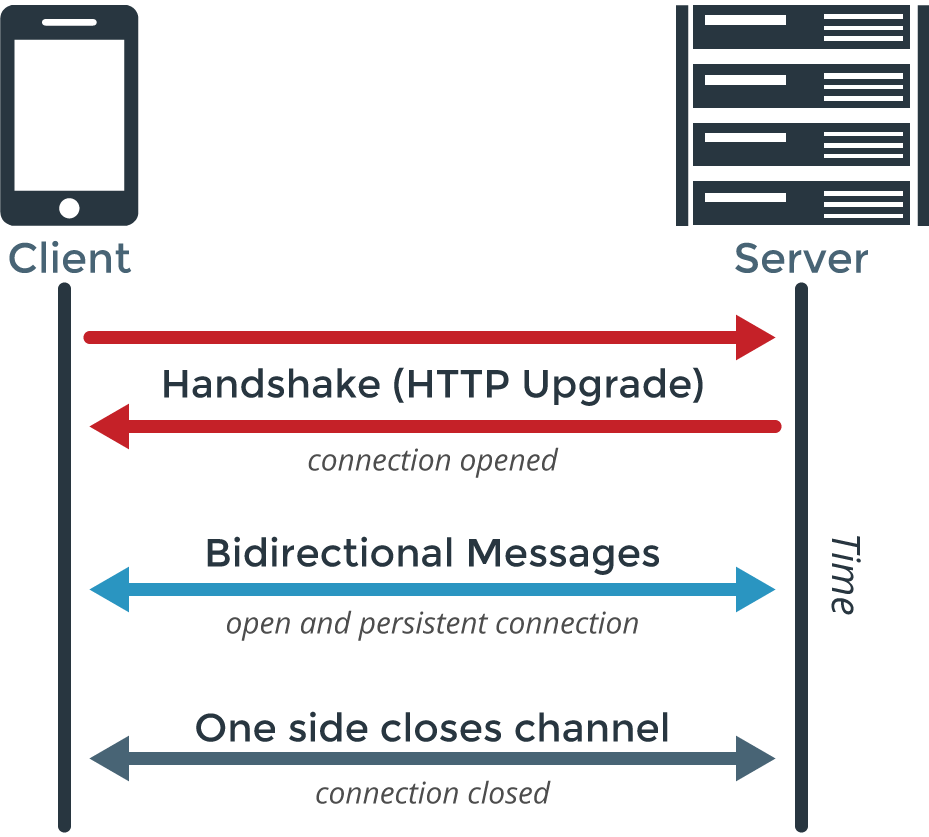
\includegraphics[width=0.45\textwidth, keepaspectratio=true]{websockets-diagram}
	\centering
	\caption[Diagrama de conexão via websocket]{Diagrama de conexão via websocket}
	\fonte{\url{https://www.pubnub.com/learn/glossary/what-is-websocket/}{}}
	\label{fig:websocket-diagram}
\end{figure}
\FloatBarrier


\subsection[\textit{SQL}]{\textit{SQL}}\label{sql}
Structured Query Language, ou comumente conhecida como SQL é uma linguagem padrão de banco de dados. 
Diferentemente das outras linguagens de banco de dados a consulta em SQL especifica a forma do resultado e não o caminho para chegar nele. Uma outra
grande diferença é que a linguagem SQL é declarativa diferindo mais uma vez das outras linguagens que por sua vez são procedurais \cite{ref-sqlhisto}.

O MySQL é um sistema de gerenciamento de banco de dados que utiliza a linguagem SQL. Atualmente é o sistema mais popular em gerenciamento de 
banco de dados. Sua rápida popularização deve-se a fácil comunicação entre servidor e aplicação.

\subsection[\textit{Fritzing}]{\textit{Fritzing}}\label{fritzing}
O \textit{Fritzing} é uma iniciativa \textit{open source} que inicialmente foi
designada a desenvolvedores amadores. Em poucas palavras
a plataforma auxilia os desenvolvedores por meio de uma interface gráfica nas primeiras montagens com Arduino
ou outro microcontrolador, sua intuitiva interface proporciona ao usuário uma rápida montagem do circuito em protoboard. O \textit{software} vai além
e permite com que os desenvolvedores tenha uma visão tanto da protoboard, como do esquemático elétrico. 


\section[\textit{Componentes Físicos}]{\textit{Componentes Físicos}}\label{comp-fisico}
No decorrer do desenvolvimento do \textit{hardware} fez-se uso de alguns componentes eletrônicos e microcontrolador que serão descritos nessa seção.
\subsection[\textit{ESP8266}]{\textit{ESP8266}}\label{esp}
É um SOC que é produzido por um fabricante chinês - Espressif - que tem como principal vantagem a comunicação \textit{Wi-Fi} já integrada em seu circuito.
O chip teve seu auge em 2014 quando "estourou" na cultura \textit{maker} com o ESP-01 (\autoref{fig:esp8266}), essa placa permite que microcontroladores se conectem a uma rede
sem fio  fazendo conexões TCP/IP, tendo a capacidade de ser servidor ou cliente \cite{ref-esp8266h}.

\begin{figure}[h!]
	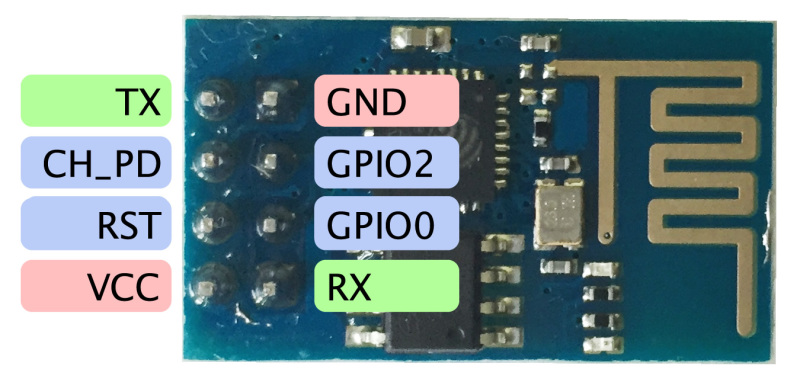
\includegraphics[width=0.3\textwidth, keepaspectratio=true]{esp8266}
	\centering
	\caption[ESP8266]{ESP8266}
	\fonte{\url{http://fabacademy.org/archives/2015/doc/images/esp-01.jpg}{}}
	\label{fig:esp8266}
\end{figure}
\FloatBarrier

O NodeMcu, \autoref{fig:nodemcu}, é uma plataformade de desenvolvimento \textit{open source}. Tem como principal linguagem de script Lua, foi construído sobre o SDK ESP8266.
A plataforma surgiu pouco tempo após o lançamento do ESP8266 (\autoref{esp}). A plataforma ganhou visibilidade, pois trazia um conjunto
de circuitos já previamente embutido que o ESP8266 por si só não proporcionava.

\begin{figure}[h!]
	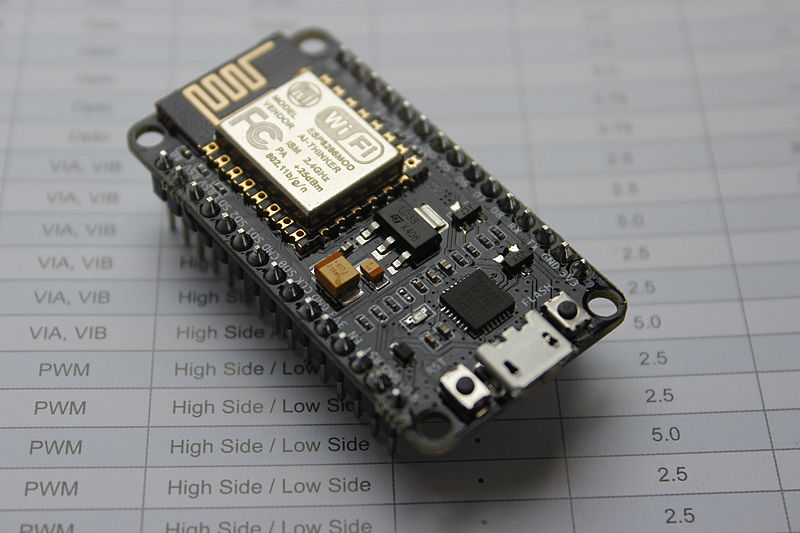
\includegraphics[width=0.4\textwidth, keepaspectratio=true]{nodemcu}
	\centering
	\caption[NodeMCU]{NodeMCU}
	\fonte{\url{https://upload.wikimedia.org/wikipedia/commons/7/7e/NodeMCU_DEVKIT_1.0.jpg}{}}
	\label{fig:nodemcu}
\end{figure}
\FloatBarrier

\subsection[\textit{Sensor de Corrente SCT 013-000}]{\textit{Sensor de Corrente SCT 013-000}}\label{sct}
O Sensor é um transformador de corrente para leituras não invasivas, possuindo um funcionamento similar a de um alicate amperímetro. Com a seguinte especificação
técnica: 
\begin{itemize}
	\item 100A no primário;
	\item Saída de 50mA no secundário;
	\item Temperatura máxima \ang{70}C;
	\item Temperatura mínima \ang{-25}C.
\end{itemize} 
Para realizar a leitura da corrente sem a necessidade de contato elétrico, o sensor de corrente alternada utiliza as propriedades 
magnéticas da corrente elétrica. O SCT, \autoref{fig:sct}, é um sensor do tipo Transformador de Corrente, que resumidamente é um conjunto de espiras que são
colocadas ao redor do condutor ao qual se quer medir a corrente. 

\begin{figure}[h!]
	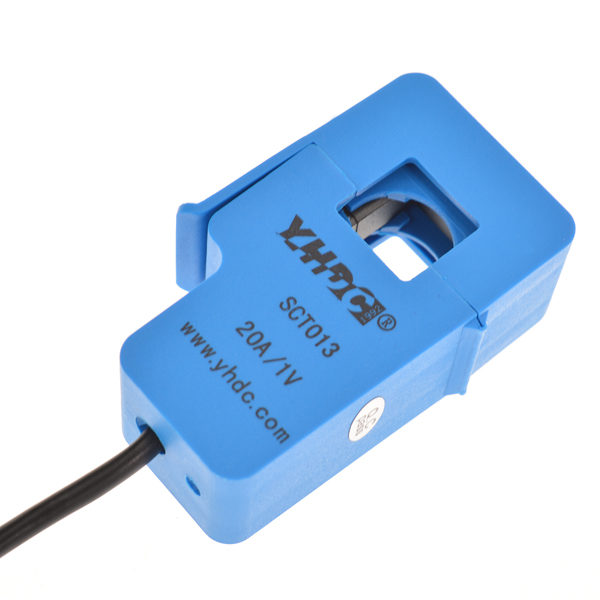
\includegraphics[width=0.3\textwidth, keepaspectratio=true]{sct}
	\centering
	\caption[SCT-013-000]{SCT-013-000}
	\fonte{\url{https://uploads.filipeflop.com/2017/07/1-34.jpg}{}}
	\label{fig:sct}
\end{figure}
\FloatBarrier
